\section{The Tiered Cascade Hybrid (TCH)}
\label{sec:cascade}

The cascade is the project's central technical contribution. It is a four-layer composition that assigns each of the seven pipelines to the sub-task it is best at and defines precisely how the layers feed each other. This section explains the design choice behind each layer, the math of the combination rule, what the layer inputs and outputs are, and how the final output is assembled.

\subsection{Design principle --- cheap and broad first, expensive and narrow last}

The cascade is ordered by per-call cost. The cheapest computations (gradient-boosted classifier on a 94-dimensional vector, a logistic-regression stacker on six scalars) run on every window. The expensive computation (the 30-second LLM agent) runs only at training/preprocessing time and only on the hardest windows.

\begin{figure}[h]
\centering
\begin{minipage}{0.97\linewidth}
\small
\begin{verbatim}
                  INPUT:  one 5-minute telemetry window
                          (logs, traces, metrics, k8s events,
                           94 derived numeric features,
                           visible Jira memory at time t)

                    +----------------------+
                    |  Six pipelines run   |
                    |  upstream + cached   |
                    | (HGB, BiEnc, HRRF-r, |
                    |  HRRF-LLM, LogSeq,   |
                    |  KG-ret)             |
                    +----------+-----------+
                               |
       +-----------------------+--------------------+-----------------+
       |                       |                    |                 |
       v                       v                    v                 v
  +---------+         +-------------------+    +----------+    +---------------+
  |   L1    |         |        L2         |    |    L3    |    |      L4       |
  | TRIAGE  |         |    RETRIEVAL      |    | NOVELTY  |    | COMPOSITION   |
  | GATE    |         |     FUSION        |    |  CHECK   |    |               |
  |         |         |                   |    |          |    | pack into:    |
  | LogReg  |         | POS 1: BiEnc top3 |    | OR of:   |--->| triage_score  |
  | over 6  |         |  + overlap rerank |    |  agent   |    | top-5 IDs     |
  | triage  |         |  (votes from      |    |  free    |    | is_novel      |
  | scores, |         |   HRRF, LogSeq)   |    |  learned |    |               |
  | 5-fold  |         |                   |    |          |    |               |
  | CV      |         | POS 2-5: RRF over |    |          |    |               |
  |         |         |  4 retrievers     |    |          |    |               |
  | tau=0.5 |         |  (k=60, top-10)   |    |          |    |               |
  +---------+         +-------------------+    +----------+    +---------------+

  OPTIONAL +-------------------------------+
  LLM PATH | DiagnosisAgent (Qwen 35B)     |
  (run at  | 3 stages: hypothesize ->      |---feeds the agent_novel
   train   | retrieve -> verify; ~30 s/win |   signal into L3
   time on +-------------------------------+
   all 1008
   test
   windows)
\end{verbatim}
\end{minipage}
\caption{The TCH cascade. Six pipelines feed four layers; L1 gates triage, L2 produces ranked retrievals, L3 flags novelty, L4 composes the final output. The agent on the right is the only inference-time LLM and feeds only the L3 novelty channel.}
\label{fig:tch-arch}
\end{figure}

\subsection{L1 --- the triage gate}

\paragraph{Job.} Decide whether the window is real or noise. Output: a calibrated probability $P(\text{ticket\_worthy}) \in [0, 1]$.

\paragraph{Architecture.} A class-balanced logistic regression \emph{stacker}. The features are the six per-pipeline triage scores; the model fits the coefficient vector $w \in \mathbb{R}^6$ and bias $b \in \mathbb{R}$ such that

\[
z = \sum_{i=1}^6 w_i x_i + b, \qquad P(\text{ticket\_worthy}) = \sigma(z) = \frac{1}{1 + e^{-z}}.
\]

\paragraph{Why a stacker and not just the best component?} HGB alone reaches strict PR-AUC $= 0.9998$, so the strict metric is essentially saturated by HGB. The other five pipelines contribute on \emph{borderline-class} windows where HGB alone is uncertain: stacking adds $+3.2$ points absolute on the inclusive PR-AUC (which counts borderline as positive).

\paragraph{Training.} 5-fold \texttt{StratifiedKFold} cross-validation with \texttt{random\_state $= 42$} and \texttt{class\_weight $= $ balanced} (to compensate for the 21.6\% positive rate). Each fold's model is fit on four-fifths of the data and scores the held-out fifth, producing \emph{out-of-fold predictions} for every training window --- predictions on data the model never saw during fit, which keeps the stacker honest. The five fold models are then averaged for inference on the held-out test set.

\paragraph{Learned coefficients.} HGB dominates with coefficient $+8.221$, roughly $30\times$ the next-largest. KG-Retrieval contributes $+0.525$; BiEncoder $+0.292$; LogSeq2Vec $+0.116$; Hybrid-RRF-LLM $+0.112$; Hybrid-RRF-rule $-0.048$ (the small negative is a regularization artifact). The bias is $-4.755$. Removing HGB from the stacker collapses strict PR-AUC from 0.9998 to 0.303, confirming HGB is essential.

\paragraph{Decision threshold.} We picked $\tau = 0.5$ by sweeping $\{0.2, 0.3, 0.5\}$ on validation: at every threshold, recall stays at 1.000 (HGB never produces false-negative scores below 0.5 on \texttt{ticket\_worthy} windows), so we choose 0.5 for the tightest precision (F1 = 0.986).

\begin{figure}[h]
\centering
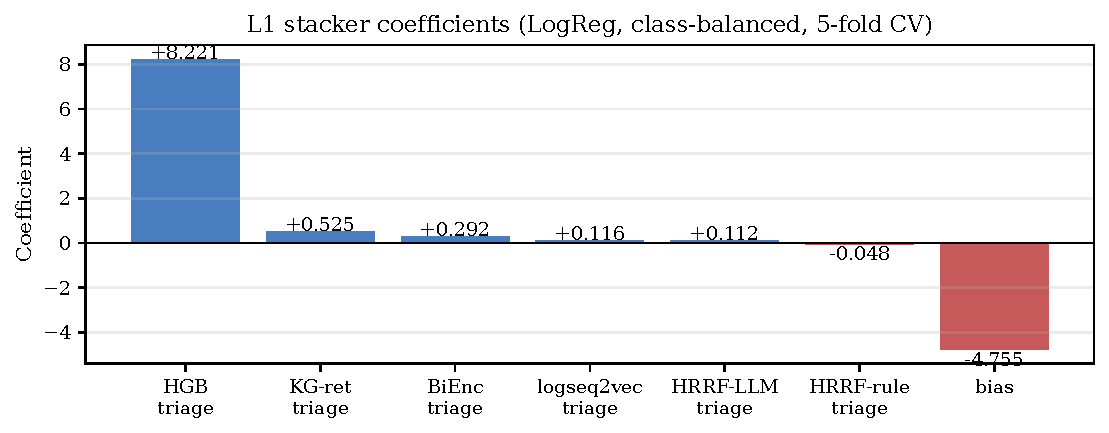
\includegraphics[width=0.9\linewidth]{figures/l1_stacker_coefs.pdf}
\caption{Learned L1 stacker coefficients. HGB dominates with $+8.221$, approximately $30\times$ the next-largest. The five other pipelines contribute small but non-zero weights, most of which is realized on borderline-class windows where the inclusive PR-AUC metric picks up the lift.}
\label{fig:l1-coefs}
\end{figure}

\subsection{L2 --- the retrieval fusion}

\paragraph{Job.} Produce a ranked top-5 of past Jira tickets that look most similar to this window. The trick is that top-1 and top-5 are different optimizations: top-1 rewards a single confident pick, top-5 rewards diverse coverage. L2 uses two different combination rules, one for each.

\paragraph{Position 1 --- anchor plus overlap rerank.}

The anchor is BiEncoder's top-3 (it has the best standalone Hit@1). For each candidate $c$ in BiEncoder's top-3, we count how many of the other retrievers also rank $c$ highly:

\[
\text{overlap}(c) = \sum_{r \in \{\text{HRRF-rule, HRRF-LLM, LogSeq2Vec}\}} w(c, r), \qquad w(c, r) = \begin{cases} 3 - \text{rank}_r(c) & \text{if } c \in \text{top3}(r), \\ 0 & \text{otherwise.}\end{cases}
\]

The candidate with the maximum overlap score wins position 1. If no candidate has any overlap, we default to BiEncoder's top-1.

\paragraph{Intuition.} A candidate that multiple independent retrievers agree on is more likely to be correct than the top-1 of any single retriever. Hit@1 climbs from BiEncoder's $0.695$ to the cascade's $0.722$.

\paragraph{Positions 2--5 --- Reciprocal Rank Fusion.}

For each retriever $r \in \{\text{BiEncoder}, \text{HRRF-rule}, \text{LogSeq2Vec}, \text{KG-Retrieval}\}$ (four retrievers, not six), and each candidate $c$ in that retriever's top-10:

\[
\text{RRF}(c) = \sum_r \frac{1}{60 + \text{rank}_r(c)}
\]

Sort candidates by $\text{RRF}(c)$ descending; remove the anchor (already at position 1); take the next four. The RRF constant $k = 60$ is from the original Cormack et al. paper, confirmed optimal on our $\{30, 60, 90, 120\}$ sweep.

\paragraph{Why exactly these four retrievers?} A drop-one ablation against the six-retriever baseline showed that \emph{removing} Hybrid-RRF-LLM \emph{improves} Hit@5 by $+2.1$ points absolute. This is the RRF density paradox we saw at the single-pipeline level recurring at the fusion level: the LLM graph produces sparse, high-precision top-10s that dilute the RRF vote. We also dropped the V2 SOTA pipeline (essentially free; no change). The remaining four contribute non-trivially: dropping BiEncoder costs $-5.7$ points, dropping LogSeq2Vec costs $-5.1$ points, dropping KG-Retrieval costs $-1.5$ points, dropping HRRF-rule is approximately zero (we keep it for redundancy).

\paragraph{Why uniform RRF instead of score-weighted RRF?} We tested several weighting schemes (weight by standalone Hit@5, weight by per-window triage confidence, learned per-candidate ranker) and every variant hurt by 4--6 points Hit@5. We also computed the \emph{per-family oracle}: if at retrieval time you knew the gold scenario family and could pick the single best retriever for that family, the resulting Hit@5 would be $0.888$ --- \emph{worse} than uniform RRF's $0.912$. Multi-retriever consensus catches windows that no per-family expert could.

\subsection{L3 --- the novelty check}

\paragraph{Job.} Emit a Boolean \texttt{is\_novel} flag when the window has no good past match. Output: a single bit.

\paragraph{Architecture --- three independent signals OR-combined.}

\[
\text{is\_novel} = \text{agent\_novel} \;\lor\; (\max_{i} \text{confidence}_i < 0.5) \;\lor\; (P_{\text{learned}}(\text{novel}) \geq 0.50)
\]

The three disjuncts are independent and complementary:

\begin{enumerate}
\item \textbf{Agent signal.} The DiagnosisAgent's verify-stage \texttt{is\_novel} output. In the final cascade the agent has run on all 1{,}008 test windows (the G4 refinement of Section~\ref{sec:experiments}). Standalone precision $= 0.94$, standalone recall $\approx 35\%$.
\item \textbf{Free signal.} \texttt{max retrieval confidence $< 0.5$}. If none of the retrievers is more than half-confident in any candidate, the window is unlikely to have a good past match. Empirically 96\% precise; costs zero LLM inference.
\item \textbf{Learned signal (the G7 contribution).} A logistic regression with class\_weight=balanced trained on 46 features per window via 5-fold StratifiedKFold cross-validation:
\begin{itemize}
\item \texttt{window\_type} one-hot (4 levels: active\_fault, observation\_window, pre\_fault\_baseline, recovery\_window)
\item \texttt{scenario\_family} one-hot (27 levels)
\item \texttt{service\_name} one-hot ($\sim$12 levels)
\item \texttt{is\_hard\_case} Boolean
\item \texttt{max\_retrieval\_conf} scalar
\item \texttt{triage\_score} scalar
\end{itemize}
The top learned coefficients are exactly what one would expect: \texttt{window\_type=pre\_fault\_baseline} weighs $+2.90$ (novel by construction --- there is no incident yet), \texttt{window\_type=recovery\_window} weighs $-2.28$ (post-incident, the gold is recent), \texttt{scenario\_family=ad-outage} weighs $+2.62$ (sparsely covered family), \texttt{scenario\_family=productcatalog-outage} weighs $-1.99$ (well-covered family). The classifier is exploiting structural metadata signal that the original fixed-threshold L3 was ignoring.
\end{enumerate}

The disjunction means a window is flagged novel if \emph{any} of the three signals fires. Operators can tune the trade-off by changing the learned-signal threshold (the cascade exposes this knob).

\paragraph{What L3 deliberately does NOT do.} L3 does not reorder L2's top-5. We tested allowing the agent to override L2's top-1 on 200 windows: the agent was right on 3, L2 was right on 8, both wrong on 9 --- a net $-5$ Hit@1 wins. On this dataset, multi-retriever consensus on top-1 dominates any single LLM judgment. L3 contributes only the novelty Boolean.

\subsection{L4 --- output composition}

\paragraph{Job.} Pack the three outputs into the final result object. No math; just dictionary assembly.

\[
\text{output} = \{\texttt{triage\_score}: P_{L1}, \;\texttt{matched\_issue\_ids}: \text{top-5}_{L2}, \;\texttt{is\_novel}: \text{flag}_{L3}\}.
\]

\paragraph{Triage decision.} A coarser \texttt{triage\_decision} field is derived from \texttt{triage\_score} via the L1 threshold: \texttt{ticket\_worthy} if $\geq 0.5$, else \texttt{noise}. Downstream products consume the calibrated probability or the Boolean depending on use case --- a triage UI might show the probability with a confidence band; a Jira-suggest dropdown might show the top-5 regardless of the triage probability; an alert system might key off \texttt{is\_novel}.

\subsection{A worked example end-to-end}

Consider a real test window: at timestamp $t$, the \texttt{paymentservice} began returning HTTP 500 at $10\times$ baseline rate and \texttt{checkoutservice}'s p99 latency spiked from 200 ms to 4 s.

\paragraph{Step 1 (pre-cached, upstream).} The six pipelines run independently and write their per-window predictions:
\begin{itemize}
\item HGB triage $= 0.97$ (numeric features highly anomalous)
\item BiEncoder top-1 $= $ \texttt{TICKET-paymentservice-unavailable-r01}, triage $= 0.61$
\item HRRF-rule top-1 $= $ same ticket, triage $= 0.71$
\item HRRF-LLM top-1 $= $ \texttt{TICKET-paymentservice-deadline-r02}, triage $= 0.68$
\item LogSeq2Vec top-1 $= $ first ticket, triage $= 0.42$
\item KG-Retrieval top-1 $= $ first ticket, triage $= 0.55$
\end{itemize}

\paragraph{Step 2 (L1).} The six triage scores feed the stacker:
\[
z = 8.221 \cdot 0.97 + 0.525 \cdot 0.55 + 0.292 \cdot 0.61 + 0.116 \cdot 0.42 + 0.112 \cdot 0.68 - 0.048 \cdot 0.71 - 4.755 \approx 3.24.
\]
$\sigma(3.24) \approx 0.962$. Decision: \texttt{ticket\_worthy}.

\paragraph{Step 3 (L2 position 1).} BiEncoder's top-3 is $[\texttt{unavailable-r01}, \texttt{deadline-r02}, \texttt{checkout-restart-r03}]$. Overlap scores:
\begin{itemize}
\item \texttt{unavailable-r01}: HR-rule ranks 1 (weight 3), HR-LLM 4 (weight 0), LogSeq ranks 1 (weight 3) $\rightarrow$ \textbf{overlap 6}
\item \texttt{deadline-r02}: HR-rule 3 (weight 1), HR-LLM 1 (weight 3), LogSeq 5 (weight 0) $\rightarrow$ overlap 4
\item \texttt{checkout-restart-r03}: HR-rule 2 (weight 2), HR-LLM 5 (weight 0), LogSeq 2 (weight 2) $\rightarrow$ overlap 4
\end{itemize}
Position 1: \texttt{paymentservice-unavailable-r01}.

\paragraph{Step 4 (L2 positions 2--5).} Compute RRF$(c)$ across the four retrievers' top-10s; remove the anchor; take the next four. Final top-5: $[$\texttt{unavailable-r01, deadline-r02, checkout-restart-r03, payment-oom-r04, frontend-timeout-r05}$]$.

\paragraph{Step 5 (L3).} Free signal: $\max \text{conf} = 0.71 \geq 0.5$, so not novel. Agent signal (post-G4): not novel. Learned signal: $P_{\text{learned}} = 0.18 < 0.50$, not novel. Final \texttt{is\_novel} $= $ \texttt{False}.

\paragraph{Step 6 (L4).} Assembly:
\begin{lstlisting}[basicstyle=\ttfamily\scriptsize]
{
  "window_id":      "production-2026-06-04-paymentservice-deadline-T123456Z",
  "triage_score":   0.962,
  "triage_decision":"ticket_worthy",
  "matched_issue_ids": [
     "TICKET-paymentservice-unavailable-r01",
     "TICKET-paymentservice-deadline-r02",
     "TICKET-checkoutservice-restart-r03",
     "TICKET-paymentservice-oom-r04",
     "TICKET-frontend-timeout-r05"
  ],
  "is_novel": false
}
\end{lstlisting}

\subsection{How the layers feed each other --- a concise summary}

\begin{table}[h]
\centering
\caption{Information flow between layers.}
\label{tab:layer-flow}
\small
\begin{tabularx}{\linewidth}{l X X}
\toprule
Layer & Reads & Writes \\
\midrule
L1 & Six pipelines' triage scores (cached) & \texttt{triage\_score} $\in [0,1]$ \\
L2 & The four chosen retrievers' top-10 ranked lists (cached) & \texttt{matched\_issue\_ids[5]} \\
L3 & L2's max retrieval confidence, the cached agent \texttt{is\_novel} output, and 46 window-level features & \texttt{is\_novel} $\in \{T, F\}$ \\
L4 & L1's \texttt{triage\_score}, L2's top-5, L3's \texttt{is\_novel} & Final output dict \\
\bottomrule
\end{tabularx}
\end{table}

The layers do not interfere: L3 never reorders L2's ranking, L2 never feeds back into L1, L1's threshold does not gate L2 (we always produce a top-5 even on noise-classified windows, so that downstream tools can show the top-5 as a sanity check). This independence is what makes the per-layer ablations clean and what made the G-series refinements safe to integrate one at a time.
